\outline{1}{Chapter 4}
\chapter{Compensation and Restitution of Post-Stroke Movement Patterns}
\label{cha:armeospring}

In this chapter, I present my study on the ArmeoSpring kinematics data.

\section{ArmeoSpring Overview}
\label{sec:overview}

The ArmeoSpring is a rehabilitation exoskeleton, designed for the purpose of ``functional arm and hand therapy''.\footnote{\label{aowebsite}https://www.hocoma.com/usa/us/products/armeo/armeospring/, last accessed 2/16/2017} 
The device is based on research and development of David Reinkensmeyer at the University of California, Irvine (UCI) and the Rehabilitation Institute of Chicago (RIC). 
Shown in figure \ref{fig:armeo}, the exoskeleton has 7 degrees of freedom (DoF), summarized in table \ref{tab:devicedof}. 
It is attached to the arm by two or three velcro straps. 
The exoskeleton has two springs equipped, at the upper arm and forearm respectively. 
The springs can be adjusted to compensate the gravity force of the arm. 
The lengths of the exoskeleton are adjustable, as well as the strength of the springs. 
There are no motors at any joints, the user has to move actively to control the exoskeleton. 
The user's trunk is mildly constrained by the velcro strap at the upper arm. 

\begin{figure}
	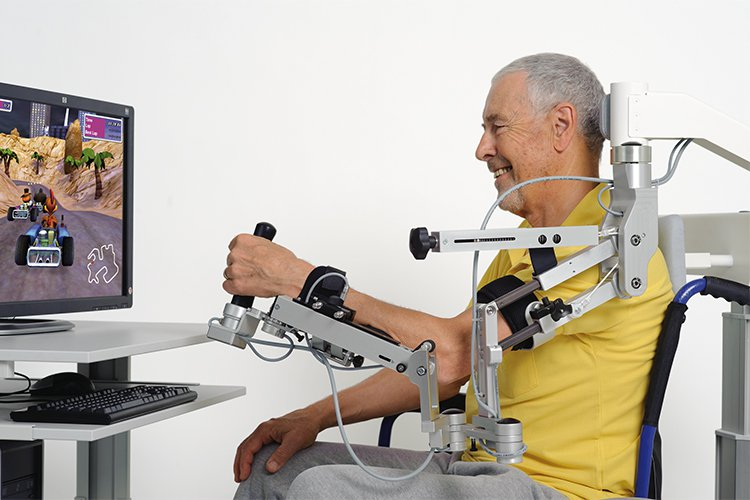
\includegraphics[width=0.5\textwidth]{armeo.jpg}
	\centering
	\caption{ArmeoSpring exoskeleton}
	\label{fig:armeo}
\end{figure}

\begin{table}
	\begin{tabular}{c c c c}
	\hline
	Joint No. & Joint Name & Anatomical Counterpart & Direction \\
	\hline
	1(1) & Inner Shoulder Angle & Shoulder Horizontal Ab-/Adduction & Left/Right \\
	1(2) & Outer Shoulder Angle & Shoulder Horizontal Ab-/Adduction & Left/Right \\
	2 & Upper Arm Angle & Shoulder Flex-/Extension & Up/Down \\
	3 & Elbow Angle & - & Left/Right \\
	4 & Forearm Angle & - & Up/Down \\
	5 & Pro-/Supination Angle & Pro-/Supination & - \\ 
	6 & Flex-/Extension Angle & Wrist Flex-/Extension & - \\
	\hline
	\end{tabular}
	\caption{Degrees of freedom of ArmeoSpring exoskeleton.}
	\label{tab:devicedof}
\end{table}

The device records all joint angles (that is, the joints of the exoskeleton), and calculates the end effector location through a forward kinematics model of the exoskeleton. 
The end effector location then is used to control a cursor on a screen, often displayed vertically in front of the user. 
The stick at the end point is equipped with a force sensor. 
During a training session, the user plays several 2D or 3D games; after a certain game, the user is often presented with performance feedbacks of that game.
Some games have difficulty settings that physical therapists can change at the beginning of a training session.

The ArmeoSpring claims to be the ``preferred therapy choice for arm and hand rehabilitation of the widest range of patients"\footnotemark[\ref{aowebsite}]. 
The lack of motors enables self-initiated movement therapy. 
The device records all joint angles and end effector trajectories, as long as task-specific variables, which helps provide assessments and document patient progress.

\section{Data Collection, Acquisition and Preprocessing}
\label{datacollect}

\subsection{Ladybug pointing test}

The ladybug pointing test (see figure \ref{fig:ladybug}) is a game in which the user tries to catch ladybugs that appear one by one pseudo randomly on a vertical screen in front of the user. 
The game is two-dimensional; the movement along the dimension perpendicular to the screen is ignored. 
To catch the ladybug, the user moves the cursor to its location. After a ladybug is caught, or a certain amount of time if not caught, the ladybug disappears and the next ladybug appears somewhere else. 
We choose this game as a test of performance because we have access to the time and location of the beginning and the end of each movement (if the ladybug is caught).%, namely from the current ladybug to the next.

\begin{figure}
	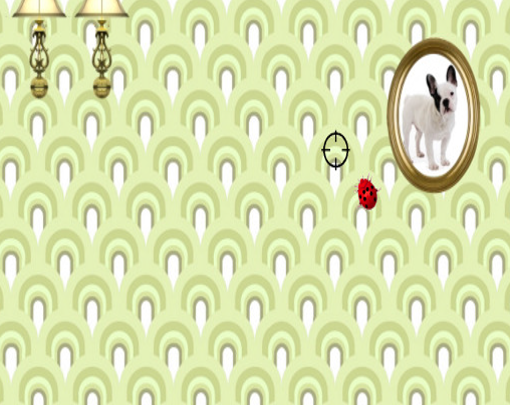
\includegraphics[width=0.5\textwidth]{ladybug.png}
	\centering
	\caption{Ladybug pointing test}
	\label{fig:ladybug}
\end{figure}

This pointing test is scheduled at the beginning and the end of each training session. For the control group (young adults, see below), each session lasts about 20 minutes. 
Two training sessions are scheduled per day in the morning and the afternoon, for 5 consecutive days. 
As a result, each subject has 10 training sessions, 20 ladybug pointing tests. 

For the control group, all games are set to be at the most difficult level. 
Specifically, the ladybug pointing test is set at level 4 in which 48 ladybugs appears sequentially. 
Though the locations of ladybugs seem to be random, they actually appears in a specific sequence at specific locations. 
At level 4, all ladybugs appear on a $6\times8$ grid, in the sequence shown in \ref{fig:48order}. (the sequences at level 1,2 and 3 are also shown.) 

\begin{figure}
	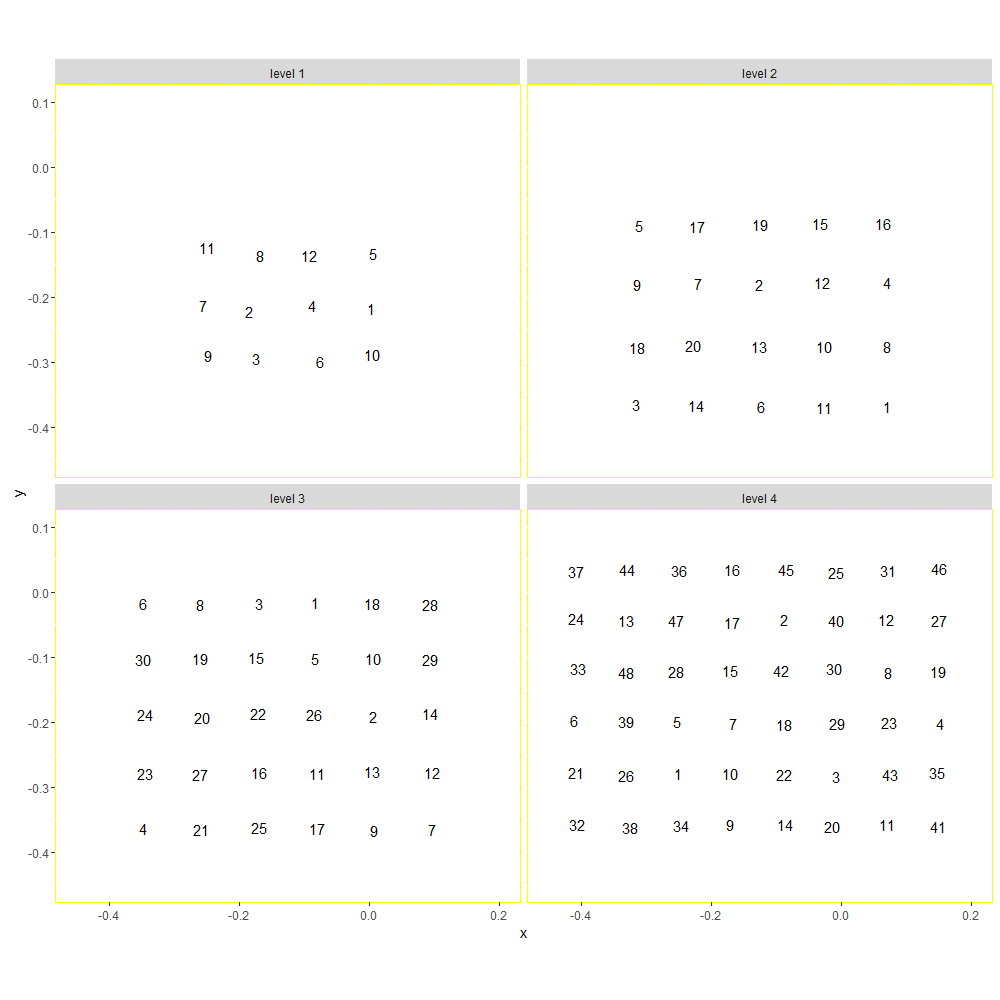
\includegraphics[width=0.8\textwidth]{48order.png}
	\centering
	\caption{Ladybug test difficulty levels and target sequence}
	\medskip
	\small The number indicates the order of the ladybug appearing at that location. The distance between adjacent targets is about 8 cm.
	\label{fig:48order}
\end{figure}

As a result, the data consists movements that have various starting positions, distances and directions.

\subsection{Control group and post-stroke group}

We recruited 11 young (age 23 $\pm$ 2) healthy subjects (7 males) to play the games which are designed for rehabilitation.

Data from post-stroke individuals are collected automatically when participants use ArmeoSpring under guidance from physical therapists. 
We have no control over game difficulty, arm length and gravity compensation settings. 
All participants have similar schedules as the control group: there are two training sessions in a day, for four weeks, weekends excluded. Therefore each participant has 40 sessions, 80 ladybug pointing tests.

We have access to data from 52 post-stroke individuals; gender and affected side are balanced, shown in table \ref{tab:demog} [need update after new subjects added]. 

\begin{table}[b]
	\begin{tabular}{c c c c c c c c}
	\hline
	Group & No. & Age & Affected Side & Gender & FM(0-66) & Post Stroke Days & No. of Tests\\
	\hline
	Stroke & 41 & 61$\pm$14 & 21L, 20R & 16F, 25M & 26$\pm$9 to 41$\pm$ 14 & 21$\pm$10 & 80 in 4 weeks \\ 
	Control & 11 & 23$\pm$2 & - & 4F, 7M & - & - & 20 in 1 weeks \\
	\hline
	\end{tabular}
	\caption{Participants information}
	\label{tab:demog}
\end{table}

Because participants have different difficulty settings from each other, and each participants may also has various difficulty settings throughout the training, it is important to see the test in different difficulty settings. 
The ladybug test under more difficult settings has larger number of ladybugs to catch, shorter time to catch the bug before it disappears, and bigger the workspace. 
In figure \ref{fig:48order}, configurations of all levels of difficulty are shown. 

The length of the exoskeleton and the strength of the springs also vary, both within and across participants.


\section{Performance in Task Space}

The kinematics data collected by ArmeoSpring can be viewed as two folds: joint angle trajectories, and end point trajectories. 
However, these two subsets are not independent since the endpoint trajectories can be derived through forward kinematics from the joint trajectories. 
Indeed that is how the end effector data is generated. 
Nevertheless, the end effector trajectories give us valuable insights regarding to each individual's performance.

The ladybug pointing test is a game rendered on a 2D vertical screen. 
To move perpendicularly to the screen has no effect on the test performance. 
In this section, I present the performance of both groups on this 2D task space.

The kinematics data are filtered with a second order Butterworth filter with a cutoff frequency of 5 Hz.

\subsection{Kinematics performance measures}

Figure \ref{fig:controlTrajExamp} shows an example of end effector trajectories before and after training, from one representative participant [sb=2] in the control group. 
The green star indicates the first ladybug of that test. 
The movement that leads to the catch of the first ladybug is discarded. 
One can immediately see the differences: the trajectories at the last test are more straight and have less over-shooting. 
This will be confirmed in section \ref{}. 
Participants in the control group never miss a target.
In contrast, figure \ref{fig:improverTrajExamp} shows an example from one participant [sb=16] in the post-stroke group. 

We performed a variety of kinematics measures on this set of end effector trajectories data. 
They can be grouped in three groups: 1) Time and duration measure; 2) Curvature and smoothness measure; 3) Movement planning [and/or execution measure]. 



\begin{figure}
	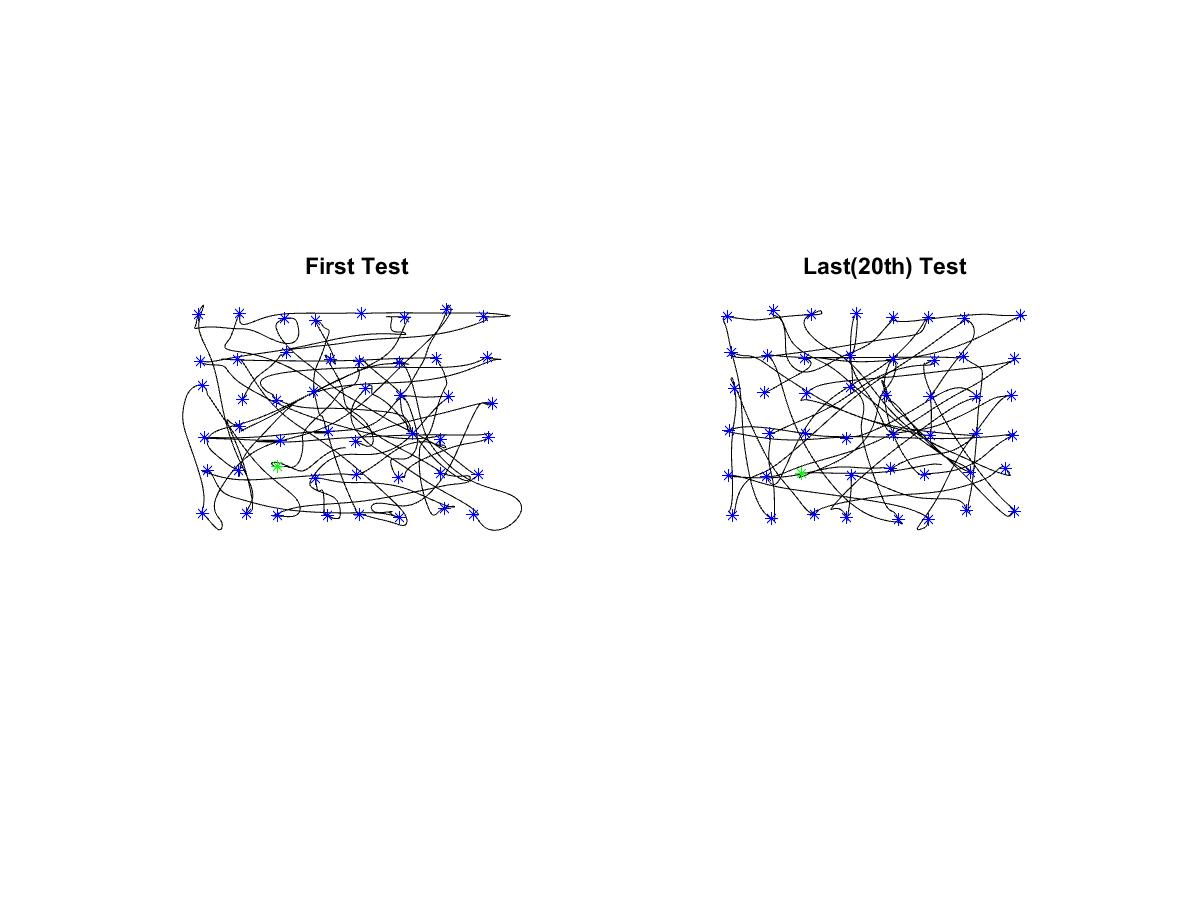
\includegraphics[width=\textwidth]{controlTrajExamp}
	\centering
	\caption{Example trajectories from control group}
	\medskip
	\small The green star is the first target
	\label{fig:controlTrajExamp}
\end{figure}

\begin{figure}
	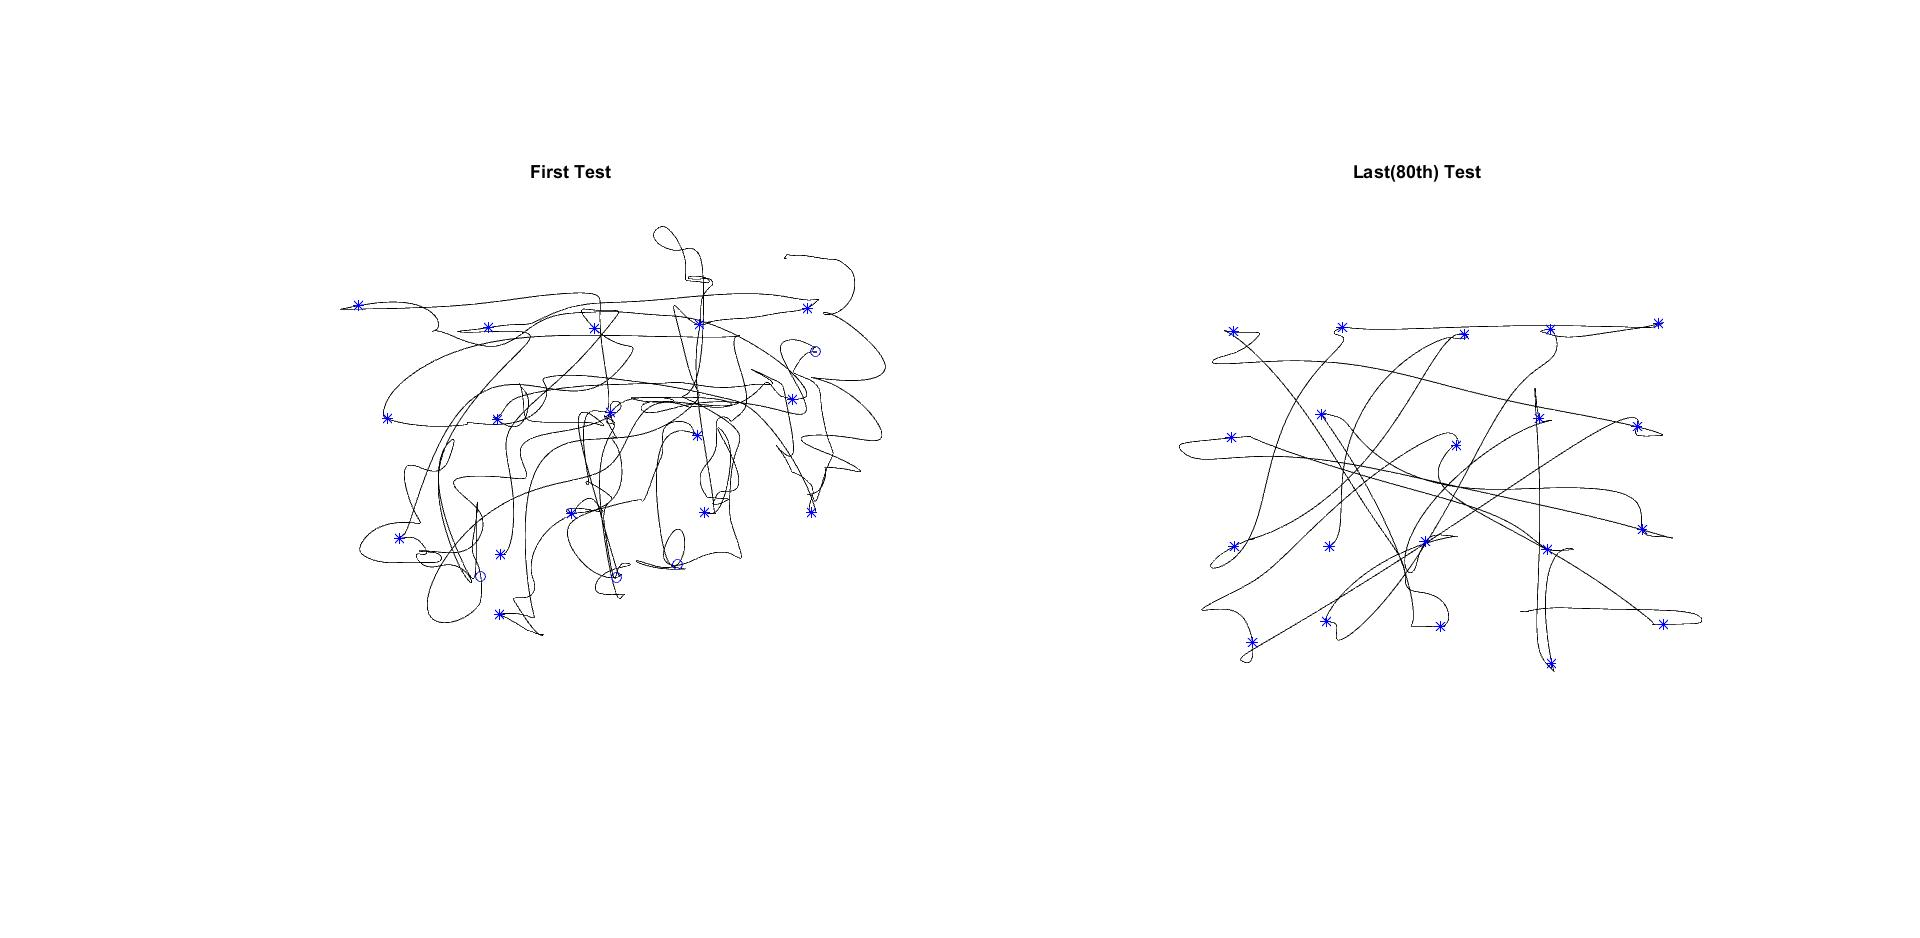
\includegraphics[width=\textwidth]{improverTrajExamp}
	\centering
	\caption{Example trajectories from post-stroke group}
	\medskip
	\small Circles are the locations of the cursor when targets disappear.
	\label{fig:improverTrajExamp}
\end{figure}

\subsubsection{Time and duration measure}
Movement duration (MD) is the time period for the execution of the reaching movement. 
The calculation of MD should be done carefully since the onset and offset of the movement is not readily available. 
A threshold is often used to determine the two, but in ArmeoSpring data, the user doesn't necessarily reach to zero velocity upon the target, so a threshold does not work very well. 
Instead we parse the movement according to the catch of the ladybug. 

An equivalent measure to MD is average speed (SPE), defined as the distance between targets divided by MD. 
This is not to be confused with average tangential velocity (VEL), which is defined as the total length of traveled path divided by MD. 
The former is a measure of movement efficiency, while the latter of movement capacity. 

Due to the fact that in ArmeoSpring data, the movements have different movement distances, and different level of tests have different average distances as well, we choose average speed as a measure of movement efficiency, and average velocity as a measure of movement capacity. 

\subsubsection{Curvature and smoothness measure}
Human movement is smooth to the extent of elegance [ref]. 
There are many approaches to measure curvature and smoothness.

Path ratio (pr) is defined as the total length of traveled path divided by the distance between targets. 
Since the denominator is surely smaller or equal to the numerator, pr is larger than or equal to (though very rare) one. 
Note that pr is also the ratio between average speed and average velocity. 
We can also define other measures in similar spirit of pr, e.g. deviation index [ref], defined as the ... and deviation area index, defined as the ... . However, pr is simply defined, robust and is immune to special cases\footnote{both deviation index and deviation area index fail at special cases, such as...}. 

Another way to evaluate movement smoothness is to look at velocity profile, which is the tangential velocity plotted against time. 
A well executed movement shows bell curve profile [ref], in which case there is only one peak. 
When the movement is not as smooth, more than one peaks can be identified. 
Therefore, number of peaks (nop) of velocity profile is also a measure of smoothness. 
However, This measure is very prune to data preprocessing, e.g. data filtered with different filter settings would give different nop. 
A similar measure is to look at number of sub modules [ref]. We choose nop for its simplicity.

Yet another group of measures concerns the jerk of the movements. 
The jerk is defined as the third derivative of the trajectory against time. 
Similar to velocity profile, it is a time series. 
The famous minimum jerk model of movements [ref] minimize jerk, as an integration of jerk over movement period. 
Maximum jerk is also worth looking at. 
Since jerk is dependent on movement duration and distance in a nontrivial way, [ref] proposes normalized jerk which is normalized against duration and distance. 
Similar to nop, jerk also is prune to data preprocessing.

\subsubsection{Movement planning and/or execution}
It is not easy to infer the quality of movement planning solely through kinematics data.
Still, some aspect of movement planning manifest itself in end effector trajectories.
Initial direction error is defined as the angle between the line connecting targets, and the line connecting .... This measures how ...[ref]. 
Feedforward ratio is defind as .. [ref]




\subsection{Performance of the Control Group}

In this section, I present the performance of the control group as measured by methods introduced in previous section. The main purpose is to estimate a baseline performance learning curve, to be compared, as a standard, with stroke group. Overall, participants in the control group show less cross-subject variance, comparing to the stroke group \ref{}. 

\textit{Method and Notations.} For each kinematics measure (take velocity $VEL$ for example), I first calculate the average $VEL$ and standard error within each test $\sigma_{VEL}$, and then calculate the group average $VEL_\textsf{group} = \textsf{mean}(VEL)$ and standard deviation $\sigma_{VEL_\textsf{group}} = \textsf{std}(VEL)$ aross participants.

\subsubsection{Tangential velocity}
The tangential velocity ($VEL_\textsf{control}$) and average speed ($SPE_\textsf{control}$) of the control group is shown in figure \ref{fig:velControlAve}. Speed and velocity are highly correlated with each other, but the gap between them decreases slightly in time (which is also shown by path ratio in \ref{}). Note that $VEL$ increases faster at the beginning, and slows down at later stage of training. This feature is also shown in the following measures.

\begin{figure}
	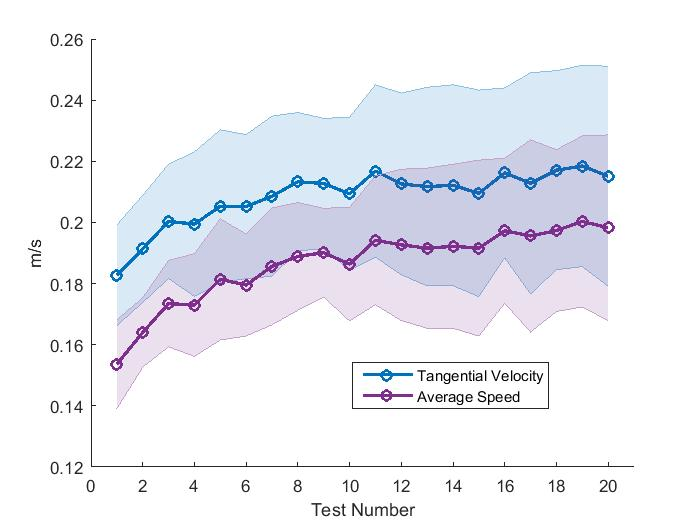
\includegraphics[width=0.7\textwidth]{velControlAve.jpg}
	\centering
	\caption{Tangential Velocity and Average Speed of control group}
	\medskip
	\small The shade represents standard deviation.
	\label{fig:velControlAve}
\end{figure}

\subsubsection{Smoothness}
We choose path ratio (pr), number of peaks (nop) and normalized jerk (nj) as a measure of smoothness. The group average data is shown in figure \ref{}. Note that the variability across subject is not very big. nop can be very well captured by linear mixed effect model. exponential model is inferior. 

\subsection{Performance of the Stroke Group}

Compared with the control group, data from the stroke group present much more variablity, both within and across participants. The data is made more complex by the fact that each participant may have different difficulty settings through out the training. So it is important to investigate the stroke group in more detail than the control group.

\subsubsection{Demographic data}

We have access to participants' age, gender, affected side, time of stroke and two clinical assessments before and after training: Fugal-Mayer score [ref] (upper extremity) and ARAT [ref]. The distribution of age, gender, affected side and time of stroke is shown in figure \ref{fig:demoData}. Figure \ref{fig:FMARAT} shows FM and ARAT of participants before and after training.

\begin{figure} % /ArmeoSpring Project/user settings/plotDemographic.R
	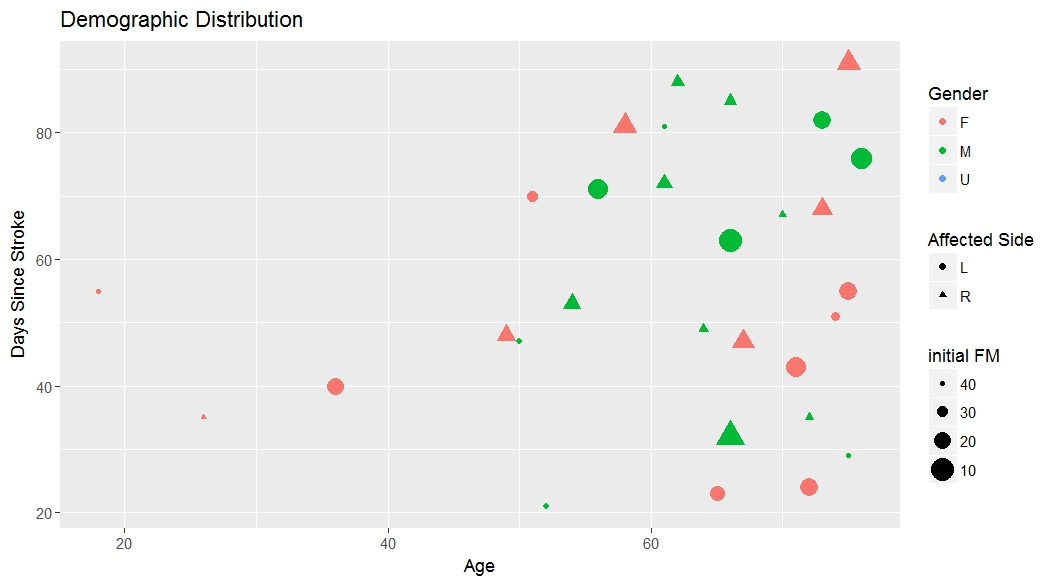
\includegraphics[width=\textwidth]{demoData.jpeg}
	\centering
	\caption{Demographic Distribution}
	\medskip
	\small 
	\label{fig:demoData}
\end{figure}

\begin{figure} % /ArmeoSpring Project/user settings/plotDemographic.R
	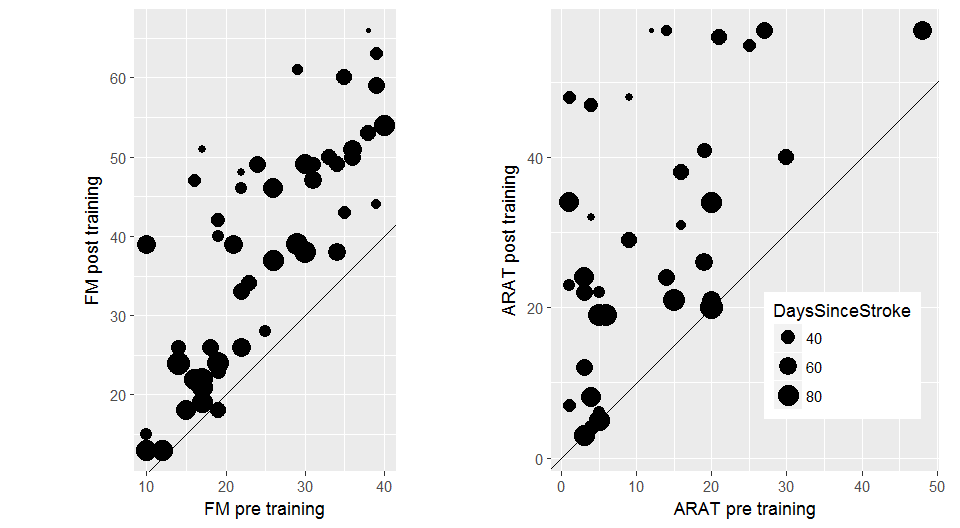
\includegraphics[width=\textwidth]{FMARAT.png}
	\centering
	\caption{FM and ARAT before and after training}
	\medskip
	\small 
	\label{fig:FMARAT}
\end{figure}

\subsubsection{Test difficulty settings}

As shown above, there are 4 levels of difficulty setting available for stroke participants. Figure \ref{fig:diffLevel} shows two examples how this difficulty setting changes through the training. As shown, not every participants share the same pattern, some of them (at least 17 participants) have no difficulty level changes, others have very small changes, as the second example in Figure \ref{fig:diffLevel}. Since the diffculty settings only have two effects: increased number of targets and enlarged workspace (shown in Figure \ref{fig:48order}), the former is accounted for by taking test average, the latter is accounted for by analysis of target locations. Hence we don't further investigate the effects of difficulty levels.

\begin{figure}
	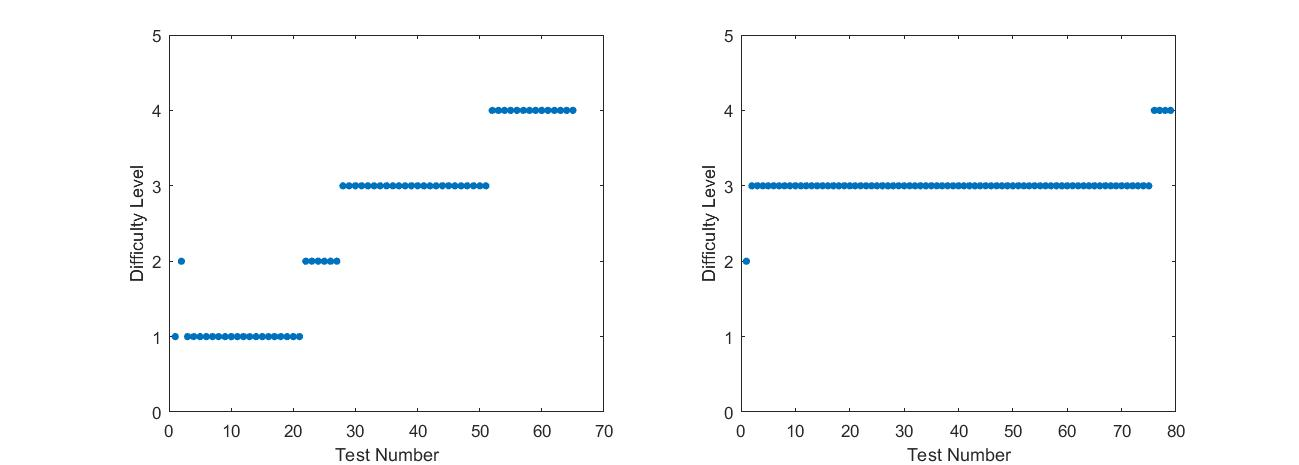
\includegraphics[width=\textwidth]{diffLevel.jpg}
	\centering
	\caption{Example difficulty settings}
	\medskip
	\small 
	\label{fig:diffLevel}
\end{figure}

\subsubsection{Successful rate}

Unlike the control group, participants in the stroke group don't usually achieve 100\% successful rate, which is defined as the percentage of targets that are successfully caught by the cursor. 


\section{Joint Coordination}

\subsection{Joint Angle Data Overview}
Although the device has seven degrees of freedom (as shown in \ref{tab:devicedof}), the first two degrees of freedom both contributes to shoulder horizontal abduction/ adduction movement, therefore they essentially degenerate into one degree of freedom.

The joints of the device do not represent anatomical joints, nevertheless, three device joints can be mapped to anatomical joints directly: Shoulder Angle $\,\to\,$ Shoulder Horizontal Ab-/Adduction, Upper Arm Angle $\,\to\,$ Shoulder Flexion/ Extension, Wrist Flexion/ Extension Angle $\,\to\,$ Wrist Flexion/ Extension. Pro-/Supination Angle of the device is not the anatomical pro-/supination angle, though they are highly correlated.


\subsection{[to-write](Attempt to)Get Joint Angles from Machine Joint Angle Recordings }
\subsection{[to-write]Pros and Cons of Dimensionality Reduction Method for Synergy Abstraction}
\subsection{[to-write]Relationship with Performance in Task Space}
